\chapter{Introduction}
In this work, the design and implementation of a social networking platform for designers of Multi-Cloud applications is presented. In this targeted social networking platform, DevOps~\cite{loukides2012devops} and particularly cloud deployment specialists can benefit from other users' experience and answer design questions such as which is the most cost-effective deployment and which configuration fits their needs.  DevOps consists of several types of specialists such as programmers, testers, QA staff and specialists from Operations who all use tools for various purposes like building applications, testing, deploying routines, configuration, automation of utilities, tracking and versioning in systems.  
Cloud Deployment Specialists are responsible for migration and configuration of hosted solutions for applications. Furthermore, they have deep industry knowledge about security, auto scaling, storage, load balancers, CDN and everything related to your application secured hosting and scalability. They talk to each other and exchange opinions on cloud deployment of applications, but the lack of a repository where they can find the configuration of an application that fits their needs.

This social network targets the cloud deployment specialists and binds all social networking concepts such as personal messaging, groups, new feeds with modelling-driven concepts of application composition and deployment, integrating a repository of cloud applications and infrastructure description based on Cloud Application Modelling and Execution Language (CAMEL)~\cite{paasagedeliverable212}. 

This CAMEL repository means to several benefits to the DevOps community.
Among the range of possible DevOps tasks, the Social Network focuses on selecting the most appropriate deployment
configuration for an application. This is especially challenging in a multi-cloud setting due to the
large diversity of deployment possibilities and tradeoffs. Currently DevOps users work with a small set of
well-understood deployment options, missing opportunities for improving performance, reliability and/or
lower cost. Investigating new options involves timeconsuming testing over new infrastructures. Discussing
with the community in online social or technical forums may provide insight over deployment options;
however the answer to a hard question often needs to be backed by experimental data that is not readily
available. 

An integrated environment can enrich user interactions with structured references to applications and their components, execution data, and mined knowledge from real deployments. Mined knowledge can be combined with user activity and profiles to provide personalized suggestions and hints.  An improved mode of user interaction is expected to result to stronger incentives for DevOps users to contribute information to the underlying repositories. More content should lead to better quality of mined knowledge, benefiting the DevOps community and providing further incentive for contributions.  The social networking platform designed to be closely integrated with a set of information repositories satisfying the following requirements: 
(R1) handle entire applications rather than just software components; (R2) abstract application structure through software modeling; (R3) capture and analyze application runtime performance. Raising the level of abstraction from components to applications. The analysis of application execution data can provide answers to many interesting questions of the community and support discussions and arguments with hard data. 
These requirements can provide software developers with strong incentives to contribute, leading to the sustainability and growth of information and derived knowledge in the repository.


%\section{Motivation}

\section{Background}
Application models inside social network platform are described in CAMEL. CAMEL integrates various domain-specific languages (DSLs). These DSLs cover a wealth of aspects of specification and execution of multi-cloud applications like CloudML, Scalability rules, WS Agreement, Saloon and Historical Execution Data. CAMEL is using the Eclipse Modelling Framework (EMF) on top of the Connected Data Objects (CDO). Applications is persisted on CDO repository.
CloudML~\cite{FerryRossiniCMS13} is a recent approach that focuses on the provisioning and deployment of multi-cloud applications, is built upon MDE techniques and methods, and provides a models@run-time environment for enacting the provisioning.  WS Agreement~\cite{andrieux2007web} is a Web Services protocol for establishing agreement between two parties, such as between a service provider and customer. Saloon ~\cite{quinton2013towards} is an approach that uses models to represent clouds variability, as well as ontologies to describe the heterogeneous aspect of the cloud ecosystem. The CAMEL model couple together aAll those DSLs as shown in figure~\ref{fig:dsls}.

Chef \ldots


\begin{figure}[h]
	\caption{CAMEL DSLs.}
	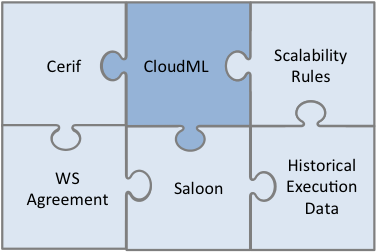
\includegraphics[width=0.6\textwidth,natwidth=200,natheight=150]{./fig/dsl.png}
	\centering
	\label{fig:dsls}
\end{figure}

%\section{Methodology}

%\section{Other section}
